
\subsection{Analityczne wyznaczanie krzywych dyspersji}

Zależności dyspersyjne są trudne, a często niemożliwe do wyznaczenia w sposób analityczny. Dla prostych przypadków rozwiązania analityczne są znane, a kilka z nich jest poniżej opisanych w celu lepszego wyjaśnienia zjawiska dyspersji.
Pierwszym przypadkiem będzie model nieskończenie długiej, napiętej sprężyny, przedstawionej na rysunku \ref{fig:nieskonczenie_krotki_odcinek_sprezyny}.

\begin{figure}[h]
\centering
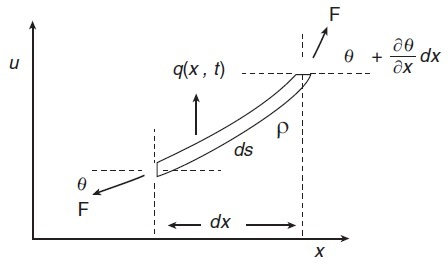
\includegraphics[width=10cm]{Zdjecia/2/dyspersja_analitycznie_sprezyna}
\caption{Nieskończenie krótki odcinek napiętej sprężyny \cite{bartek_rose}}
\label{fig:nieskonczenie_krotki_odcinek_sprezyny}
\end{figure}

Symbole z rysunku oznaczają:

\begin{eqwhere}[2cm]
        \item[$ds$] długość sprężyny
        \item[$\theta$] kąt przyłożenia siły zewnętrznej
        \item[$F$] siły wewnętrzne
        \item[$q$] siła oddziaływania sprężyny na jednostkę długości ugięcia
        \item[$\rho$] masa sprężyny na jednostkę długości.
\end{eqwhere}

Korzystając z drugiej zasady dynamiki Newtona, zapisujemy równanie ruchu układu:

\begin{equation}
-Fsin\theta+Fsin(\theta+\frac{\partial \theta}{\partial x}dx)+qds = \rho ds \frac{\partial^2u}{\partial t^2}.
\end{equation}

Załóżmy dodatkowo, że:

\begin{equation}
ds \approx dx\; ,\; sin\theta=\theta \; i\; \theta = \frac{\partial u}{\partial x}.
\end{equation}

To pozwala uprościć równanie:

\begin{equation}
-F\theta+F(\theta + \frac{\partial \theta}{\partial x}dx)=\rho dx\frac{\partial^2 u}{\partial^2 t}
\end{equation}

\begin{equation}
F\frac{\partial^2 u}{\partial x^2} + q = \rho \frac{\partial^2 u}{\partial^2 t}.
\end{equation}

Jeśli założymy brak siły zewnętrznej, to otrzymujemy proste równanie falowe:

\begin{equation}
\frac{\partial^2 u}{\partial x^2} = \frac{1}{c_0^2} \frac{\partial^2 u}{\partial^2 t},\quad c_0=\sqrt{\frac{F}{\rho}}
\end{equation}

gdzie
\begin{eqwhere}[2cm]
        \item[$c_0$] prędkość fali.
\end{eqwhere}

Przyjmijmy rozwiązanie w postaci:

\begin{equation}
u(x,t)=Ae^{i(kx-\omega t)}.
\end{equation}

Jeśli wstawimy je do równania falowego to otrzymamy zależność dyspersyjną:

\begin{equation}
\omega^2=c_0^2 k^2.
\end{equation}

Jest to przypadek liniowej zależności \( k(\omega)\), a więc dyspersja fali nie zachodzi. W takim przypadku prędkość fazowa, jest równa prędkości grupowej:

\begin{equation}
V_p=\frac{\omega}{k}=\frac{d\omega}{dk}=V_g
\end{equation}

Prosta modyfikacja układu ze sprężyną jak na rysunku \ref{fig:nieskonczenie_krotki_odcinek_sprezyny2}, powoduje skomplikowanie zależności dyspersyjnej.

\begin{figure}[h]
\centering
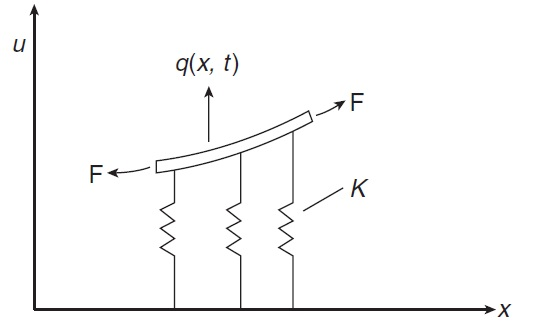
\includegraphics[width=10cm]{Zdjecia/2/dyspersja_analitycznie_sprezyna2}
\caption{Nieskończenie krótki odcinek napiętej sprężyny na sprężystym podłożu \cite{bartek_rose}}
\label{fig:nieskonczenie_krotki_odcinek_sprezyny2}
\end{figure}

Przyjmijmy siłę \(q=-Ku(x,t)\), co prowadzi do równania równowagi:

\begin{equation}
\frac{\partial^2 u}{\partial x^2} - \frac{K}{F}u = \frac{1}{c_0^2} \frac{\partial^2 u}{\partial^2 t}.
\end{equation}

Ponownie załóżmy rozwiązanie w postaci \( u(x,t)=Ae^{i(kx-\omega t)} \) i podstawmy je do równania równowagi. Prowadzi to do zależności:

\begin{equation}
\Big(-k^2-\frac{K}{F}+\frac{w^2}{c_0^2}\Big)e^{i(kx-\omega t)}=0.
\end{equation}

Równanie to jest nazywane równaniem charaktersytycznym (lub dyspersyjnym). Rozwiązaniem jest:

\begin{equation}
-k^2-\frac{K}{F}+\frac{w^2}{c_0^2}=0.
\end{equation}

Zależność \(k(\omega)\) przyjmuje postać:

\begin{equation}
k^2=\frac{w^2}{c_0^2}-\frac{K}{F}.
\end{equation}

Podstawiając \( k=\frac{\omega}{c_p}\), otrzymujemy :

\begin{equation}
c_p = \sqrt{c_0^2\Bigg( \frac{1}{1 - \frac{c_0^2 K}{\omega^2 F} } \Bigg)}.
\end{equation}

Jak widać w takim przypadku prędkość fazowa jest zależna od częstotliwości, a więc będzie zachodzić dyspersja fali.

\vspace{3mm}

Kolejnym problemem wartym wspomnienia, jest problem propagacji fal Lamba w cienkiej, nieskończonej płycie. Płyta wraz z przyjętym układem współrzędnych znajduje się na rysunku \ref{fig:nieskonczona_plyta}.

\begin{figure}[h]
\centering
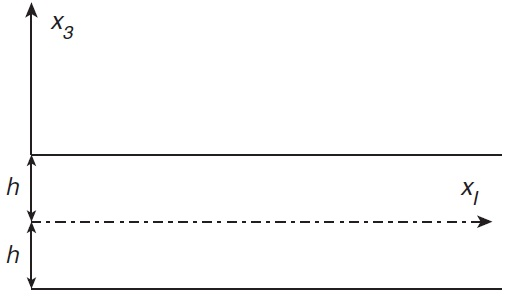
\includegraphics[width=10cm]{Zdjecia/2/dyspersja_analitycznie_plyta}
\caption{Nieskończona płyta \cite{bartek_rose}}
\label{fig:nieskonczona_plyta}
\end{figure}

Jest kilka metod rozwiązania takiego zagadnienia, ale nie są opisane one w tej pracy (metoda potencjałów, metoda fal cząstkowych). Jeśli przyjmiemy zerowe naprężenia na płaszczyznach zewnętrznych jako warunki początkowe, to związki dyspersyjne przyjmują zależności:

\begin{equation}\label{fig:RL1}
\frac{tan(qh)}{tan(ph)}=-\frac{4k^2pq}{(q^2-k^2)^2}
\end{equation}
dla postaci symetryczych oraz

\begin{equation}\label{fig:RL2}
\frac{tan(qh)}{tan(ph)}=-\frac{(q^2-k^2)^2}{4k^2pq}
\end{equation}
dla postaci antysymetrycznych,

gdzie
\begin{equation}
p^2=\frac{\omega^2}{c_L^2} - k^2 \; ,a \; q^2=\frac{\omega^2}{c_L^2}-k^2
\end{equation}

\begin{eqwhere}[2cm]
        \item[$c_T$] prędkość fali poprzecznej
	\item[$c_L$] prędkość fali podłużnej
\end{eqwhere}

Równania \ref{fig:RL1}, \ref{fig:RL2} nazywają się równaniami Rayleigha-Lamba i są nierozwiązywalne w sposób analityczny. Jest to przykład bardziej skomplikowanego modelu, gdzie możliwe jest wyznaczenie związków \(k\) i \(\omega\), ale do wykreślenia krzywych dyspersji konieczne jest zastosowanie metod numerycznych.
